\documentclass{seal_article}

\usepackage{hyperref}
\usepackage{booktabs}

\title{S.E.A.L. Article}
\subtitle{Example}

\begin{document}
\maketitle

\section{Methodology}

\subsection{Bug prediction}
The study aims to analyse the performance accuracy of cloud specific bugs using traditional bug prediction pipeline. 

\subsubsection{Project Sample}
Since we used the tool \textsc{ck} \cite{ck} to compute some of our metrics which specifically targets \textsc{Java} projects, we only included Java cloud projects in our sample. Furthermore, we selected projects with at least 100 releases.
\subsubsection{Data Preparation}
\paragraph{\textit{Metrics Selection}}
Important metrics types to feed in to bug prediction pipeline were chosen based on earlier researches on similar context.  (add a small description)

\begin{itemize}
\item loc - Counts the lines of code ignoring the empty lines.
\item cbo- Counts the number of dependencies of each class 
\item dit -  Counts the inherited classes of each class
\item wmc - Counts the number of branch instructions in a class
\item lcom - Lack of cohesion of methods
\end{itemize}

\paragraph{\textit{Data Ingestion}}
JGit is a java implementation of Git version control system. Git parser was implemented as the initial step of the bug prediction pipeline. All the commit messages between 2 releases were retrieved through the parser and then bug related commits were filtered using specific keywords to filter out the class names with the bugs.
\\Keywords to filter bugs : 
\textit{error, fix, failure, crash, unexpected, wrong}
\vspace{\baselineskip}
\textsc{CK} \cite{ck} library was used in for all the classes at the time of the release in order to retrieve the certain features to generate the metrics. CK java library provides class level and metric level code metrics without compiling the code. Above mentioned loc, cbo, dit, wmc, lcom were calculated written into the excel sheet with an extra column mentioning whether each of the class has a bug or not by going through the list of class names with bugs.

\paragraph{\textit{Data Cleaning}}
Data duplication couldn’t be handled at the level of the java code due to the limitations of the used libraries. Before feeding in to the machine learning pipeline quality and reliability of data was assured through various pre-processing steps. In this stage irrelevant and redundant data is removed. 

\subsubsection{Model Building and Training}
Logistic regression machine learning technique was chosen to build the model based on hyper parameter properties. RWeka library which is R interface of a collection of machine learning algorithms for data mining tasks written in java. 

\subsubsection{Process Diagram}
\vspace{\baselineskip}
\begin{figure}[htp]
    \centering
    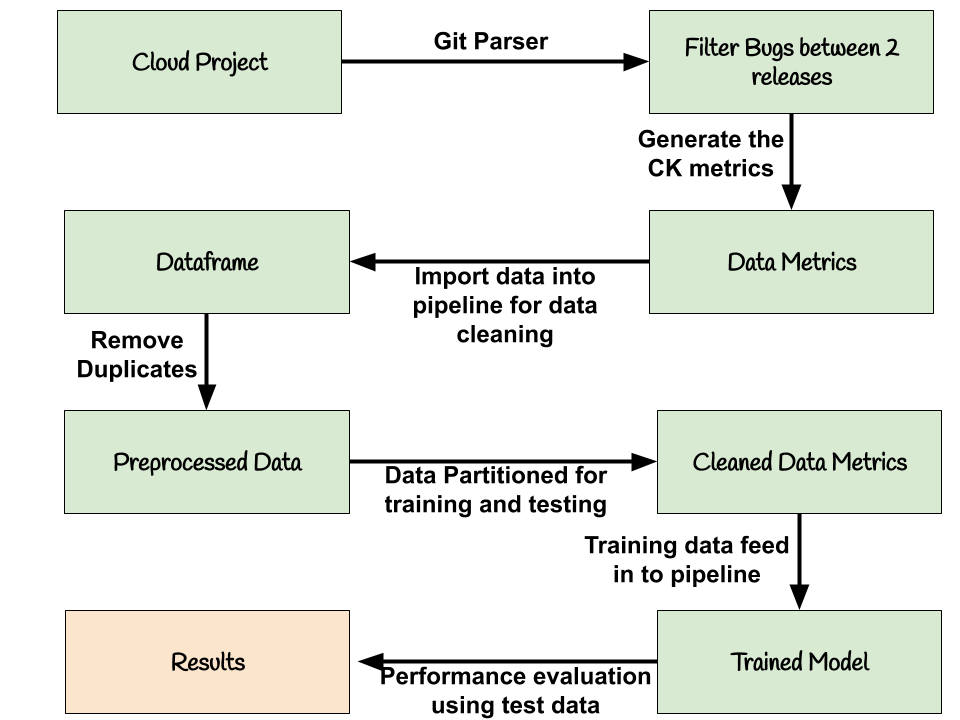
\includegraphics[width=8cm]{Process.png}
    \caption{Machine Learning Pipeline}
    \label{fig:Initial Bug }
\end{figure}


\subsection{ASAT adoption in Cloud System}
To answer RQ2, we searched for cloud applications and collected information about ASATs of the Go language. 

\subsubsection{Projects}
We created a sample of 10 cloud projects written in \textsc{Go} that use ASAT and proceeded with the collection as follows: We used \textsc{GitHub}'s search functionality\footnote{https://github.com/search} using query words such as \textit{cloud}, \textit{PaaS} or \textit{SaaS} to find suitable projects. We filtered the projects by the programming language (\textsc{Go}) and the number of stars (>500). We chose Go because it is considered a major language for cloud computing \cite{thenewstack}. We then manually checked whether a given project really represented a cloud system by reading the repository's description, e.g. we found projects that just provide a CLI to a cloud service or tools for the development of cloud projects, but are not cloud applications themselves. Finally, we removed projects that do not use ASAT using a script that scans all projects files for ASAT command usage (more details in the next section).

\subsubsection{Model building and training}



\subsubsection{ASATs}
There are more than 30 ASATs available for the Go language. We gathered these tools from a GitHub repository \cite{awesome_asat} that compiles a list of ASATs for many programming languages. We excluded some of these tools, namely those that were archived or deprecated (e.g. \cite{interfacer}), or exploratory in nature (e.g. \cite{goroutine}) as we were interested in ASATs highlighting issues in the code. We stored all ASATs in a sqlite database.

The majority of ASATs specialize on specific problems in the code such as detecting deadlocks \cite{dingo-hunter} or unused arguments in function declarations \cite{nargs}. Two ASATs in our database are linter aggregators , i.e. they run multiple ASATs \cite{goreporter,golangci-lint}. Finally, some ASATs cover a variety of code issues (e.g\cite{staticcheck}). 

Many ASATs can be configured in terms of which warnings are enabled, what files they are run on or at which thresholds a warning should be issued. These configuration settings may be passed via a file or command line arguments.

\subsubsection{Commandline configuration}


%\begin{lstlisting}[caption=An example code snippet]
%/**
% * Javadoc comment
% */
%public class Foo {
%	// line comment
%	public void bar(int number) {
%		if (number < 0) {
%			return; /* block comment */
%		}
%	}
%}
%\end{lstlisting}

\bibliographystyle{abbrv}
\bibliography{references}

\end{document}
